\documentclass[10pt,a4paper]{article}
\usepackage[margin=2.2cm]{geometry}
\usepackage{amsmath,amssymb}
\usepackage{graphicx}
\usepackage{booktabs}
\usepackage{hyperref}
\usepackage{xcolor}
\usepackage{tikz}
\usepackage{caption}
\usepackage{float}
\usepackage{microtype}
\usetikzlibrary{arrows.meta,positioning,shapes.geometric,fit,backgrounds,calc}

\hypersetup{colorlinks=true,linkcolor=blue!70!black,citecolor=blue!70!black,urlcolor=blue!60!black}

% Stage colors
\definecolor{discoverblue}{RGB}{41,128,185}
\definecolor{decideorange}{RGB}{230,126,34}
\definecolor{buildgreen}{RGB}{39,174,96}
\definecolor{operategray}{RGB}{100,120,130}
\definecolor{verifypurple}{RGB}{142,68,173}
\definecolor{reviewteal}{RGB}{22,160,133}
\definecolor{knowledgegold}{RGB}{200,130,18}
\definecolor{policyred}{RGB}{192,57,43}
\definecolor{deliverred}{RGB}{192,57,43}
\definecolor{l0color}{RGB}{52,73,94}
\definecolor{l1color}{RGB}{41,128,185}
\definecolor{l2color}{RGB}{39,174,96}
\definecolor{arrowgray}{RGB}{120,120,120}
\definecolor{feedbackorange}{RGB}{211,84,0}
\definecolor{memoryblue}{RGB}{70,130,180}
\definecolor{evolvegreen}{RGB}{46,139,87}

\pagestyle{empty}

\begin{document}

%% ============================================================
%% MAIN BODY — AGENT SKILL ARCHITECTURE (~1 page)
%% ============================================================

\section{Agent Skill Architecture}
\label{sec:agent-architecture}

Complex scientific workflows demand agents that not only execute multi-step tasks but also learn from their own execution.
A static collection of capabilities cannot anticipate every failure mode, adapt to new domains, or close quality gaps discovered only at runtime.
We address this challenge with a meta-skills framework built on two pillars: a \emph{three-layer invocation hierarchy} that separates routing, orchestration, and atomic execution; and a \emph{closed-loop evolution mechanism} that transforms every task execution into a learning opportunity.

\paragraph{Three-layer invocation model.}
The system organizes capabilities into three layers of increasing granularity (Figure~\ref{fig:three-layer}).
\emph{Entry commands} (L0) are thin routers that accept natural-language requests---three commands (\texttt{/meta}, \texttt{/build}, \texttt{/research}) constitute the entire user-facing interface.
\emph{Path templates} (L1) are declarative YAML recipes specifying step sequences, gate requirements, and branch conditions; eight templates cover workflows from skill health audits to hypothesis-driven research.
\emph{Atomic capabilities} (L2) are 29 contract-driven building blocks with typed inputs and outputs, organized across an eight-stage lifecycle (Discover through Knowledge).
Cross-cutting \emph{quality policies} inject verification rules automatically at gate transitions based on artifact types, decoupling what the agent can do, how it sequences actions, and when it enforces quality.
A visibility boundary hides all internal layers behind \texttt{\_}-prefixed directories; users see only three commands.

\paragraph{Design principles.}
Two ideas enable the system to grow without destabilizing.
First, components are separated by \emph{change rate}: L0 commands are frozen, L2 capabilities evolve rapidly in hidden directories, and policies evolve slowly as failure modes are codified---additions to one layer require no coordinated changes to others.
Second, constraints are enforced \emph{mechanically}: naming governance (18 controlled verbs, 91 canonical objects) is checked by validation scripts, and quality gates fire at every transition regardless of whether the agent ``remembers'' to invoke them.

\paragraph{Continuous self-evolution.}
The architecture's central contribution is a closed loop that makes the system self-improving (Figure~\ref{fig:evolution-loop}).
Every L0 command defaults to a dual-agent team: an \emph{executor} performs the user's task while an \emph{observer} (running on a cheaper model) monitors for improvement signals---policy violations, capability gaps, step deviations, repeated errors, quality misses, and automation candidates.
Overhead remains low (${\sim}1.05\times$ for simple tasks, $1.3$--$1.5\times$ for complex ones) through a complexity tiering system that adjusts observer depth.
Each finding maps to a concrete change: a new L2 capability, an L1 path adjustment, or a new \texttt{rule-*} policy.

Quality policies function as a \emph{one-way ratchet}: once a failure mode is identified, it is formalized into a policy enforced mechanically at every subsequent execution, preventing the same class of error from recurring.
Cross-session continuity relies on a three-layer memory protocol---an auto-injected summary (L1), a structured handoff document (L2), and a permanent session archive (L3)---all updated before session termination.
Observer reports feed into a recurring-patterns index that elevates repeated signals for systematic resolution, closing the loop from execution back to architecture.
The eight-stage lifecycle further supports a hypothesis-driven research pipeline (\texttt{/research}) with three feedback loops---fail-to-fix, iterate, and pivot---and a persistent hypothesis tree that accumulates results across experiments.


%% ============================================================
%% APPENDIX
%% ============================================================
\clearpage
\appendix

\section{Agent Architecture Details}
\label{app:agent-architecture}

This appendix provides detailed descriptions and figures for the agent skill architecture presented in Section~\ref{sec:agent-architecture}.


%% ------------------------------------------------------------
\subsection{Three-Layer Invocation Model}
\label{app:three-layer}

The system organizes agent capabilities into three layers of increasing granularity (Figure~\ref{fig:three-layer}).
At the top, \emph{entry commands} (Layer~0) serve as thin routers: three commands---\texttt{/meta}, \texttt{/build}, and \texttt{/research}---accept natural-language requests and match them to appropriate workflows.
Below these, \emph{path templates} (Layer~1) are declarative YAML recipes that specify step sequences, gate requirements, and branch conditions for iterative loops.
The core system defines eight such templates covering workflows from skill health audits to hypothesis-driven research.
At the base, \emph{atomic capabilities} (Layer~2) comprise 29 contract-driven building blocks, each with typed inputs and outputs, organized across an eight-stage lifecycle: Discover, Decide, Build, Verify, Deliver, Operate, Review, and Knowledge.

Cross-cutting quality policies operate independently of this hierarchy.
Rather than relying on agent judgment to decide when quality checks should run, the system injects verification rules automatically at gate transitions based on the \emph{artifact types} each step produces.
A step that emits an evidence bundle triggers reproducibility checks; a step that produces a gate verdict invokes minimum-quality thresholds.
This artifact-driven design decouples \emph{what} the agent can do (capabilities), \emph{how} it sequences actions (path templates), and \emph{when} it enforces quality (policies), enabling each dimension to evolve independently.

A visibility boundary separates the user-facing interface from internal complexity: users interact with three entry commands, while the 29 capabilities, 8 path templates, and 9 quality policies reside in directories prefixed with~\texttt{\_}, hidden from auto-discovery.


%% ============================================================
%% FIGURE 1: Three-Layer Architecture
%% ============================================================
\begin{figure}[ht]
\centering
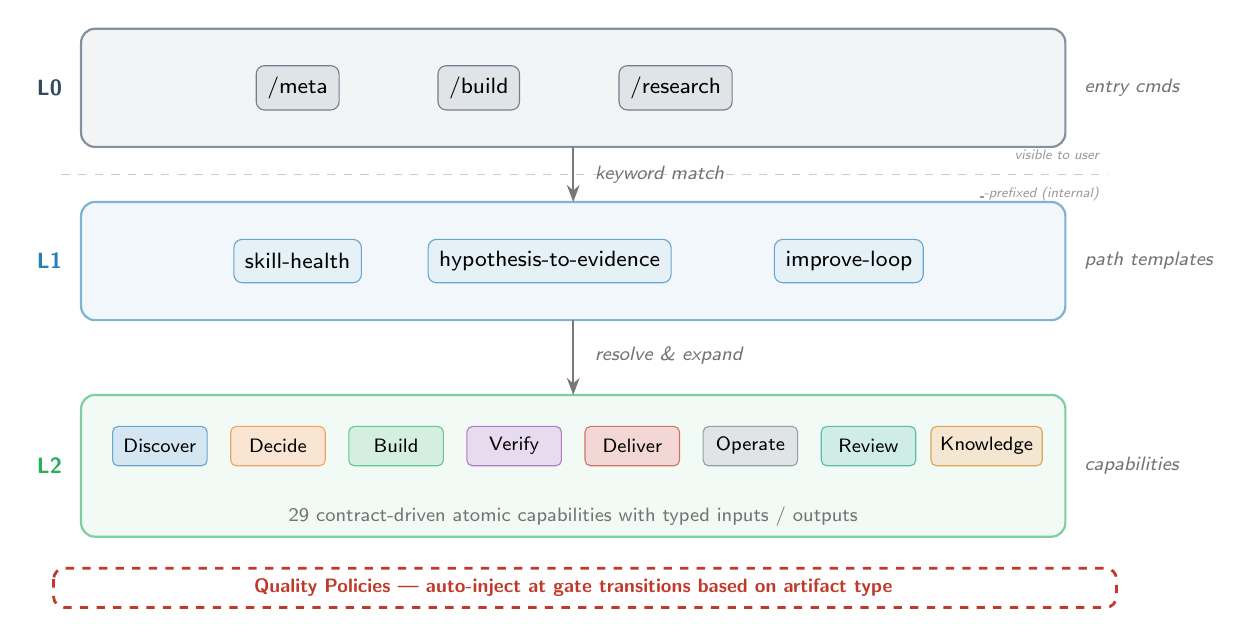
\begin{tikzpicture}[
    >=Stealth,
    band/.style={rounded corners=5pt, draw=#1!60, fill=#1!6, line width=0.8pt,
        minimum width=12.5cm, minimum height=1.5cm},
    cmdbox/.style={rounded corners=3pt, draw=l0color!70, fill=l0color!15,
        minimum height=0.55cm, font=\footnotesize\sffamily, inner sep=4pt},
    pathbox/.style={rounded corners=3pt, draw=l1color!70, fill=l1color!12,
        minimum height=0.55cm, font=\footnotesize\sffamily, inner sep=4pt},
    stagebox/.style={rounded corners=2pt, draw=#1!70, fill=#1!20,
        minimum width=1.2cm, minimum height=0.5cm, font=\scriptsize\sffamily,
        align=center},
    layerlbl/.style={font=\footnotesize\bfseries\sffamily, text=#1},
    sublbl/.style={font=\scriptsize\sffamily, text=black!55},
    arrw/.style={->, arrowgray, line width=0.7pt},
    vislbl/.style={font=\tiny\sffamily\itshape, text=black!40},
]

% === LAYER 0 (visible zone) ===
\node[band=l0color] (l0) at (0, 0) {};
\node[layerlbl=l0color, anchor=east] at ([xshift=-3pt]l0.west) {L0};
\node[cmdbox] at (-3.5, 0) {/meta};
\node[cmdbox] at (-1.2, 0) {/build};
\node[cmdbox] at (1.3, 0) {/research};
\node[sublbl, anchor=west] at ([xshift=3pt]l0.east) {\textit{entry cmds}};

% Visibility annotation
\draw[black!20, dashed, line width=0.5pt] (-6.5, -1.1) -- (6.8, -1.1);
\node[vislbl, anchor=east] at (6.8, -0.85) {visible to user};
\node[vislbl, anchor=east] at (6.8, -1.35) {\texttt{\_}-prefixed (internal)};

% === LAYER 1 ===
\node[band=l1color] (l1) at (0, -2.2) {};
\node[layerlbl=l1color, anchor=east] at ([xshift=-3pt]l1.west) {L1};
\node[pathbox] at (-3.5, -2.2) {skill-health};
\node[pathbox] at (-0.3, -2.2) {hypothesis-to-evidence};
\node[pathbox] at (3.5, -2.2) {improve-loop};
\node[sublbl, anchor=west] at ([xshift=3pt]l1.east) {\textit{path templates}};

% === LAYER 2 ===
\node[band=l2color, minimum height=1.8cm] (l2) at (0, -4.8) {};
\node[layerlbl=l2color, anchor=east] at ([xshift=-3pt]l2.west) {L2};
\node[stagebox=discoverblue]  at (-5.25, -4.55) {Discover};
\node[stagebox=decideorange]  at (-3.75, -4.55) {Decide};
\node[stagebox=buildgreen]    at (-2.25, -4.55) {Build};
\node[stagebox=verifypurple]  at (-0.75, -4.55) {Verify};
\node[stagebox=deliverred]    at (0.75, -4.55) {Deliver};
\node[stagebox=operategray]   at (2.25, -4.55) {Operate};
\node[stagebox=reviewteal]    at (3.75, -4.55) {Review};
\node[stagebox=knowledgegold, minimum width=1.4cm] at (5.25, -4.55) {Knowledge};
\node[sublbl] at (0, -5.45) {29 contract-driven atomic capabilities with typed inputs / outputs};
\node[sublbl, anchor=west] at ([xshift=3pt]l2.east) {\textit{capabilities}};

% === ARROWS L0 -> L1 ===
\draw[arrw] (0, -0.75) -- (0, -1.45);
\node[sublbl, anchor=west] at (0.15, -1.1) {\textit{keyword match}};

% === ARROWS L1 -> L2 ===
\draw[arrw] (0, -2.95) -- (0, -3.9);
\node[sublbl, anchor=west] at (0.15, -3.4) {\textit{resolve \& expand}};

% === QUALITY POLICIES (bottom strip) ===
\draw[policyred, line width=1pt, dashed, rounded corners=4pt]
    (-6.6, -6.1) rectangle (6.9, -6.6);
\node[font=\scriptsize\bfseries\sffamily, text=policyred] at (0, -6.35)
    {Quality Policies --- auto-inject at gate transitions based on artifact type};

\end{tikzpicture}
\caption{Three-layer skill invocation architecture.  Entry commands (L0) route user requests to path templates (L1), which expand into atomic capabilities (L2) organized by lifecycle stage.  A dashed visibility boundary separates the three user-facing commands from internal layers prefixed with~\texttt{\_}.  Quality policies inject automatically at gate transitions based on the artifact types produced.}
\label{fig:three-layer}
\end{figure}


%% ------------------------------------------------------------
\subsection{Design Principles}
\label{app:design-principles}

Two foundational ideas shape the architecture and enable the system to grow without destabilizing.

\paragraph{Separate components that change at different rates.}
Entry commands (L0) are frozen and rarely modified.
Atomic capabilities (L2) evolve rapidly as the system encounters new task types, and reside in hidden directories where changes cannot disrupt the user interface.
Quality policies sit between these extremes, evolving slowly as new failure modes are codified.
This \emph{stability gradient}---frozen foundation, growing middle layer, slowly-evolving guardrails---mirrors the inner/outer loop pattern from DevOps and the fixed-foundation / dynamic-capabilities / safety-guardrails structure observed in self-evolving agent architectures.
Because each layer changes at its own rate, additions to one layer do not require coordinated changes to the others.

\paragraph{Enforce mechanically, not by documentation.}
The system treats the execution environment as a \emph{harness} rather than a set of guidelines that agents may or may not follow.
Naming governance (18 controlled verbs, 91 canonical objects) is enforced by validation scripts, not by style guides.
Structural checks catch malformed capabilities before deployment.
Cross-cutting policies inject quality gates at every gate transition automatically.
This design makes violations structurally impossible rather than merely discouraged: a naming error triggers a linter failure, and a missing quality check fires regardless of whether the agent ``remembers'' to run it.


%% ------------------------------------------------------------
\subsection{Continuous Self-Evolution}
\label{app:self-evolution}

The architecture's central contribution is the closed loop that makes the system \emph{self-improving}: every skill execution feeds observations back into the system's own capabilities, policies, and knowledge (Figure~\ref{fig:evolution-loop}).
Four mechanisms form this loop.

\paragraph{Accompanied execution.}
Every L0 command defaults to a dual-agent team: an \emph{executor} that performs the user's task, and an \emph{observer} that monitors for improvement opportunities.
The observer runs on a smaller, cheaper model (Haiku) and employs signal-based monitoring rather than full-trace analysis.
This keeps overhead low: approximately $1.05\times$ for simple tasks (read, search, check) and $1.3$--$1.5\times$ for complex ones (write, build, research).
A complexity tiering system classifies commands into \emph{light} and \emph{full} tiers, with observers adapting their depth accordingly---light-tier observers perform a single post-hoc analysis, while full-tier observers monitor three checkpoints aligned with lifecycle gate transitions.

The observer watches for six high-value signal types: policy violations, capability gaps, step deviations, repeated errors, quality misses, and automation candidates.
Each finding maps to a concrete change: a new L2 capability, an L1 path adjustment, or a new quality policy.
Graceful degradation ensures that observer failures never block the user's task.

\paragraph{Policy ratchet.}
Quality policies function as a one-way ratchet.
Once accompanied execution identifies a failure mode, it is formalized into a new \texttt{rule-*} policy and enforced mechanically at every subsequent execution.
Because policies trigger based on artifact types rather than agent memory, they prevent regression deterministically---the same class of error cannot recur once the corresponding policy is in place.
Over time, the set of enforced policies grows monotonically, progressively closing quality gaps.

\paragraph{Three-layer memory.}
Cross-session continuity relies on a write-on-end protocol with three persistence layers.
Layer~1 is an auto-injected compact summary (\texttt{MEMORY.md}) that every new session receives mechanically, requiring no voluntary action.
Layer~2 is a structured handoff document (\texttt{HANDOFF.md}) read at session start, containing active TODOs, blockers, and recently modified files.
Layer~3 is a permanent session archive with timestamped records available for historical lookup.
All three layers must be updated before any session terminates; omitting any one constitutes a memory discontinuity.
Automated pruning retains the 30 most recent sessions to prevent unbounded growth.

\paragraph{Knowledge capture and pattern accumulation.}
The Review stage of the lifecycle extracts reusable principles from retrospectives and archives them as knowledge cards.
Observer reports feed into a recurring-patterns index (\texttt{PATTERNS.md}) that tracks signal types, frequencies, and resolution status across sessions.
When the same signal type recurs---for example, repeated step deviations in a particular path template---the index elevates it for systematic resolution rather than one-off repair.
This trend-detection mechanism transforms individual observations into structural improvements, closing the loop from execution back to architecture.


%% ============================================================
%% FIGURE 2: Continuous Self-Evolution Loop
%% ============================================================
\begin{figure}[ht]
\centering
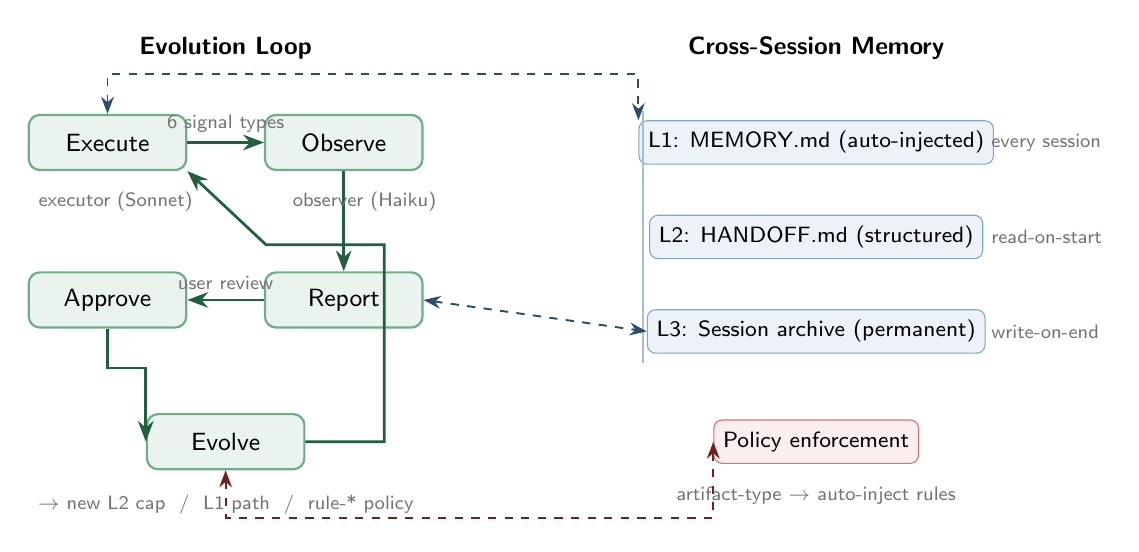
\begin{tikzpicture}[
    >=Stealth,
    loopnode/.style={rounded corners=4pt, draw=evolvegreen!70, fill=evolvegreen!10,
        minimum width=2.0cm, minimum height=0.7cm,
        font=\small\sffamily, align=center, line width=0.8pt},
    memnode/.style={rounded corners=3pt, draw=memoryblue!70, fill=memoryblue!10,
        minimum width=3.8cm, minimum height=0.55cm,
        font=\footnotesize\sffamily, align=center},
    polbar/.style={rounded corners=3pt, draw=policyred!70, fill=policyred!8,
        minimum width=2.6cm, minimum height=0.55cm,
        font=\footnotesize\sffamily, align=center},
    looparr/.style={->, evolvegreen!70!black, line width=1.0pt},
    memarr/.style={<->, memoryblue!60!black, line width=0.7pt, dashed},
    polarr/.style={<->, policyred!60!black, line width=0.7pt, dashed},
    annot/.style={font=\scriptsize\sffamily, text=black!55},
    heading/.style={font=\small\bfseries\sffamily},
]

% === LEFT: Evolution loop (circular) ===
\node[heading] at (-3.0, 3.0) {Evolution Loop};

\node[loopnode] (exec)    at (-4.5, 1.8) {Execute};
\node[loopnode] (observe) at (-1.5, 1.8) {Observe};
\node[loopnode] (report)  at (-1.5, -0.2) {Report};
\node[loopnode] (approve) at (-4.5, -0.2) {Approve};
\node[loopnode] (evolve)  at (-3.0, -2.0) {Evolve};

% Loop arrows
\draw[looparr] (exec.east) -- (observe.west)
    node[midway, above, annot] {6 signal types};
\draw[looparr] (observe.south) -- (report.north);
\draw[looparr] (report.west) -- (approve.east)
    node[midway, above, annot] {user review};
\draw[looparr] (approve.south) -- ++(0, -0.5) -| (evolve.west);
\draw[looparr] (evolve.east) -- ++(1.0, 0) -- ++(0, 2.5) -- ++(-1.5, 0) -- (exec.south east);

% Annotations on evolve outputs
\node[annot, anchor=north] at (-3.0, -2.55) {$\rightarrow$ new L2 cap ~/~ L1 path ~/~ rule-* policy};

% Dual-agent annotation
\node[annot, anchor=north west] at (-5.5, 1.3) {executor (Sonnet)};
\node[annot, anchor=north east] at (-0.2, 1.3) {observer (Haiku)};

% === RIGHT: Memory stack ===
\node[heading] at (4.5, 3.0) {Cross-Session Memory};

\node[memnode] (m1) at (4.5, 1.8) {L1: MEMORY.md (auto-injected)};
\node[memnode] (m2) at (4.5, 0.6) {L2: HANDOFF.md (structured)};
\node[memnode] (m3) at (4.5, -0.6) {L3: Session archive (permanent)};

% Stack brackets
\draw[memoryblue!50, line width=0.6pt] (2.3, 2.2) -- (2.3, -1.0);

% Memory labels
\node[annot, anchor=west] at (6.6, 1.8) {every session};
\node[annot, anchor=west] at (6.6, 0.6) {read-on-start};
\node[annot, anchor=west] at (6.6, -0.6) {write-on-end};

% === CENTER-BOTTOM: Policy enforcement bar ===
\node[polbar] (pol) at (4.5, -2.0) {Policy enforcement};
\node[annot, anchor=north] at (4.5, -2.45) {artifact-type $\rightarrow$ auto-inject rules};

% === Cross connections ===
\draw[memarr] (report.east) -- (m3.west);
\draw[memarr] (exec.north) -- ++(0, 0.5) -| (m1.north west);
\draw[polarr] (evolve.south) -- ++(0, -0.6) -| (pol.west);

\end{tikzpicture}
\caption{Continuous self-evolution loop.  \textbf{Left}: every skill execution spawns a dual-agent team; the observer detects improvement signals and proposes changes that, once approved, feed back as new capabilities, paths, or policies.  \textbf{Right}: a three-layer memory stack ensures cross-session continuity, while artifact-type-driven policy enforcement mechanically injects quality gates.}
\label{fig:evolution-loop}
\end{figure}


%% ------------------------------------------------------------
\subsection{Research Pipeline Integration}
\label{app:research-pipeline}

The eight-stage lifecycle supports a hypothesis-driven research pipeline instantiated through the \texttt{/research} command.
The pipeline transforms a research question into validated evidence through three explicit feedback loops.
Quality-gate failure returns to Build for implementation fixes.
A ``continue'' decision loops to Decide for the next iteration.
A ``change direction'' signal retreats to Discover for strategic reformulation.
Four properties underpin its effectiveness: the pipeline is \emph{hypothesis-driven} (every experiment targets a falsifiable claim), \emph{MVP-recursive} (each iteration tests one hypothesis with pre-defined acceptance thresholds), \emph{fail-fast} (consecutive failures escalate from fixes to strategic pivots), and \emph{knowledge-accumulating} (results from every experiment---including negative ones---feed into a persistent hypothesis tree).

\end{document}
